\documentclass[17pt]{beamer} %Makes presentation
%\documentclass[handout]{beamer} %Makes Handouts
\usetheme{Singapore} %Gray with fade at top
\useoutertheme[subsection=false]{miniframes} %Supppress subsection in header
\useinnertheme{rectangles} %Itemize/Enumerate boxes
\usecolortheme{seagull} %Color theme
\usecolortheme{rose} %Inner color theme

\definecolor{light-gray}{gray}{0.75}
\definecolor{dark-gray}{gray}{0.55}
\setbeamercolor{item}{fg=light-gray}
\setbeamercolor{enumerate item}{fg=dark-gray}

\setbeamertemplate{navigation symbols}{}
%\setbeamertemplate{mini frames}[default]
%\setbeamercovered{dynamics}
\setbeamerfont*{title}{size=\Large,series=\bfseries}
\setbeamerfont{footnote}{size=\tiny}

%\setbeameroption{notes on second screen} %Dual-Screen Notes
%\setbeameroption{show only notes} %Notes Output

\setbeamertemplate{frametitle}{\vspace{.5em}\bfseries\insertframetitle}
\newcommand{\heading}[1]{\noindent \textbf{#1}\\ \vspace{1em}}

\usepackage{bbding,color,multirow,times,ccaption,tabularx,graphicx,verbatim,booktabs}
\usepackage{colortbl} %Table overlays
\usepackage[english]{babel}
%\usepackage[latin1]{inputenc}
%\usepackage[T1]{fontenc}
\usepackage{lmodern}

%\author[]{Thomas J. Leeper}
\institute[]{
  \inst{}%
  Department of Government\\London School of Economics and Political Science
}

\usepackage{tikz}
\usetikzlibrary{shapes,arrows,decorations.pathreplacing,calc}

\newcounter{itemnum}

\newcommand{\nt}[2][0pt]{%
    \stepcounter{itemnum}%
    \if###2##%
    \else
        #2%
        \thinspace
    \fi
    \tikz[overlay,remember picture,baseline=(\theitemnum.base),xshift=#1]\node (\theitemnum){};%
}

\newcommand{\makebrace}[4][0pt]{%
    \begin{tikzpicture}[overlay, remember picture]
        \draw [decoration={brace,amplitude=0.5em},decorate]
        let \p1=(#2), \p2=(#3) in
        ({max(\x1+#1,\x2+#1)}, {\y1+1.75ex}) -- 
            node[right=0.6em] {#4} ({max(\x1+#1,\x2+#1)}, {\y2-0.5ex});
    \end{tikzpicture}%
}

\newenvironment{braceitems}{%
    \begin{enumerate}
}{%
    \end{enumerate}
    \setcounter{itemnum}{0}%
}


\title{Measurement:\\Concepts in Practice}

% To study something, we need to be able to observe and measure it. How do we \textit{operationalize} concepts so that we can study political phenomena? What are challenges of measuring concepts? How do we assign quantitative values to observations?

\date[]{}

\begin{document}

\frame{\titlepage}

\frame{\tableofcontents}


\section{Review}
\frame{\tableofcontents[currentsection]}


\frame{

\frametitle{Concept Definition}

\begin{itemize}
\item Classical approach
	\begin{itemize}
	\item Minimal
	\item Maximal
	\item Ordinal
	\end{itemize}
\item Family resemblance approach
\end{itemize}

}

\frame{

\frametitle{Family Resemblance}

\begin{itemize}
\item Necessary and sufficient:\\
	\hspace{1em} {\footnotesize $\text{\textbf{Rule of Law}}$}
\item Unnecessary and sufficient:\\
	\hspace{1em} {\footnotesize $\text{\textbf{Rule of Law}} \lor \text{Equality}$}
\item Necessary and insufficient:\\
	\hspace{1em} {\footnotesize $\text{\textbf{Rule of Law}} \land \text{Equality} \land Elections$}
\item Unnecessary and insufficient:\\
	\hspace{1em} {\footnotesize $(\text{\textbf{Rule of Law}} \lor \text{Equality}) \land Elections$}
\end{itemize}

}

\frame{
\frametitle{Gerring's Criteria}

\begin{enumerate}
\item Resonance (face validity)
\item Domain/scope % ladder of generality
\item Consistency
\item Fecundity
\item Differentiation
\item Causal utility
\item Operationalization
\end{enumerate}
}

% divide these up and have someone present each one


% Resonance: Is the concept intuitive? Avoid neologism (Gerring p.118); we don't need new terms for the sake of having new terms

% Domain: The contexts in which this concept resonates and applies. Example: "vouchers". What does this mean? This has a clear meaning in the United States, in debates about education policy, but that is a narrow domain. Contrast this with democracy or terrorism, which are concepts with broad domains.

% Consistency: We can change the definition of a concept by adding, removing, or modifying attributes; Contrast with "slippage" or "stretching"

% Fecundity: Fertility or fruitfulness; Neologisms are prone to lacking fecundity

% Differentiation: How does this concept contrast or help create distinctions between existing sets of phenomena? Example: *Opinion* is a summary evaluation of a particular object; *Value* is a belief about a desired end-state of the world

% Causal Utility: Concept has to be useful for making a causal argument; this may require a concept to be more specific or have higher intensity than we would prefer because we need to *use* the concept

% Operationalization: concepts have to be measurable; we'll talk about this next week





\section{Measurement}
\frame{\tableofcontents[currentsection]}


\frame{
\frametitle{An Example: Opinion}

\begin{itemize}\itemsep0.5em
\item \textit{Opinion} is a summary evaluation of a particular object
\item Only one necessary feature: evaluation/favorability
\item How do we measure this?
\end{itemize}

}

% Agree/disagree
% Oppose/support
% Degree of favorability
% Warm/cool
% Positive/negative
% How many scale points?
% Implicit: text analysis, skin conductance, heart rate, implicit association test


\frame{

\frametitle{Operationalization I}

\begin{itemize}\itemsep0.75em
\item To study concepts, we need to be able to observe those concepts
\item<2-> \textit{Operationalization} is the process of creating measures for concepts
\item<3-> Recall the definition of \textit{variable}:
	\begin{itemize}
	\item A dimension that describes an observation
	\item<4-> The operationalization of a concept
	\end{itemize}
\end{itemize}

}


\frame{

\frametitle{Operationalization II}

\vspace{-2em}

\begin{center}
\tikzstyle{block} = [rectangle, draw, fill=blue!20!white, text width=5em, text centered, rounded corners, minimum height=1em, node distance=7em]
\begin{tikzpicture}[scale=0.5]
\draw<1-> [block] node at (0,0) (concept) {{\Large Concept}};
\draw<1-> [block] node at (-5, -3) (a1) {Attribute};
\draw<1-> [block] node at (0, -3) (a2) {Attribute};
\draw<1-> [block] node at (5, -3) (a3) {Attribute};
\draw<1-> [->, very thick] (concept) -- (a1);
\draw<1-> [->, very thick] (concept) -- (a2);
\draw<1-> [->, very thick] (concept) -- (a3);

\draw<1-> [block, align=center] node at (-11.5, -1.5) (def) {Concept Definition};
\draw<1-> [decorate,very thick, decoration={brace,amplitude=10pt},xshift=-10pt,yshift=0pt]
(-7.5,-3.4) -- (-7.5,0.5);

\draw<2-> [block] node at (-5, -8) (m1) {{\small Measure(s)}};
\draw<2-> [block] node at (0, -8) (m2) {{\small Measure(s)}};
\draw<2-> [block] node at (5, -8) (m3) {{\small Measure(s)}};

\draw<2-> [->, very thick] (a1) -- (m1);
\draw<2-> [->, very thick] (a2) -- (m2);
\draw<2-> [->, very thick] (a3) -- (m3);

\draw<2-> [block, align=center] node at (-11.5, -6.5) (def) {Operation-alization};
\draw<2-> [decorate,very thick, decoration={brace,amplitude=10pt},xshift=-10pt,yshift=0pt]
(-7.5,-8.5) -- (-7.5,-3.6);


\end{tikzpicture}
\end{center}


}

\frame{

\frametitle{Operationalization III}

{\Large

Definition\\ 
	\onslide<2->{\hspace{1em} $\rightarrow$ Feature} \\
	\onslide<3->{\hspace{3em} $\rightarrow$ Indicator(s)}
}

\vspace{1em}

\onslide<4-5>{Indicators might be scaled or potential alternatives}
}


\frame{

\frametitle{Example: Democracy}

{\Large

Democracy\\ 
	\onslide<2->{\hspace{1em} $\rightarrow$ Free and fair elections} \\
	\onslide<3->{\hspace{3em} $\rightarrow$ ?}
}

\vspace{1em}
How do we operationalize this concept?
}


\frame{\huge\vskip20pt\textbf{Questions?}}


\frame{

\frametitle{Types of Measures}

\begin{braceitems}\itemsep1em
\item \nt{Categorical}
	\begin{itemize}
	\item Binary
	\end{itemize}
\item \nt{Ordinal}
\item \nt{Interval}
\end{braceitems}
\makebrace{1}{2}{Qualitative}
\makebrace{2}{3}{Quantitative}

\vspace{0.5em}

{\small Note: \textit{Ratio} scale measures are interval measures with a non-arbitrary zero value}

}

% describe difference between qualitative and quantitative
% qualitative is assigning a descriptive label
% quantitative is assigning a numerical value

% describe the three types



\frame{

\frametitle{Activity}

\begin{itemize}\itemsep0.5em
\item Concept: Democracy
\item Attribute: Free and fair elections
\item Measure:
	\begin{enumerate}
	\item Categorical
	\item Ordinal
	\item Numeric
	\end{enumerate}
\end{itemize}

}


\frame{

\frametitle{Coding}

\begin{itemize}\itemsep1em
\item Variable: A dimension that describes an observation
\item Coding: Assigning a score for a variable to an observation\\
	\begin{itemize}
	\item<2-> Manual or hand coding
	\item<2-> Automated coding
	\end{itemize}
\end{itemize}

}

% think about cases: given your measures of ``free and fair elections'', how does Britain score on each of those?



\frame{

\frametitle{{\large Using Multiple Indicators}}

\begin{itemize}\itemsep1em

\item Choose the ``best'' one

\item Apply an AND operator
	\begin{itemize}
	\item Must have all indicators to be coded 1
	\item Treat indicators as ``ordinal'' in Gerring's sense
	\end{itemize}

\item Scale the indicators (e.g., sum or mean)

\end{itemize}

}

% do you add? do you average? do you count some indicators more than others?




\frame{\huge\vskip20pt\textbf{Questions?}}



\section{Assessing Measurement Quality}
\frame{\tableofcontents[currentsection]}

\frame{

\frametitle{{\large Assessing Measurement Quality}}

\begin{enumerate}\itemsep1em
\item Conceptual clarity
\item Construct validity
	\begin{itemize}
	\item Convergent validity
	\item Divergent validity
	\end{itemize}
\item Accuracy and precision
\end{enumerate}

}

\frame{
\frametitle{Assessing Measures I}

\begin{itemize}\itemsep1em
\item Conceptual clarity is about knowing what we want to measure
\item Sloppy concepts make for bad measures
	\begin{itemize}
	\item Ambiguity % multiple meanings or multiple labels
	\item Vagueness % concept without a definition
	\end{itemize}
\item<2-> Revise concept definition as needed
\end{itemize}
}


\frame{
\frametitle{Assessing Measures II}

\begin{itemize}\itemsep0.5em
\item Construct validity is the degree to which a variable measures a concept\footnote{Note: Kellstedt and Whitten call this ``content validity''. They use ``construct validity'' to mean whether a measure has predictive validity (i.e., that the measure is related to measures of other concepts that are theorized to be related).}
\item<2-> Construct validity is \textbf{high} if a variable is a measure of the concept we care about
\item<3-> Construct validity is \textbf{low} if a variable is actually a measure of something else
\end{itemize}
}

% sources: bad concept definition; totally inappropriate measures (using income to measure weight); measure becomes the concept (actual income is replaced by self-reported income)

\frame{

\frametitle{{\large Assessing Construct Validity}}

\begin{itemize}\itemsep1em
\item Multiple measures!
\item Look for:
	\begin{itemize}
	\item Convergence (Convergent validity)
	\item Discrimination (Discriminant validity)
	\end{itemize}
\item<2-> For example, the multi-trait, multi-method matrix
\end{itemize}
}

% two (or more) measures of the same concept are highly correlated; scaling
% two (or more) measures of distinct concepts are not correlated
% Measures of distinct concepts may be correlated if they are causally related to one another, so simple correlations do not mean two measures are necessarily of the same concept

% mention predictive validity (what Kellstedt and Whitten call construct validity)




\frame<1-2>[label=challenges3]{

\frametitle{Assessing Measures III}

\Large

\begin{itemize}\itemsep1em
\item<2-> Accuracy
\item<3-> Precision
\item<4-> Reliability
\end{itemize}

}

\frame{
\frametitle{Accurate}
{\small Synonyms: true, correct, unbiased, valid}\\
\vspace{1em}

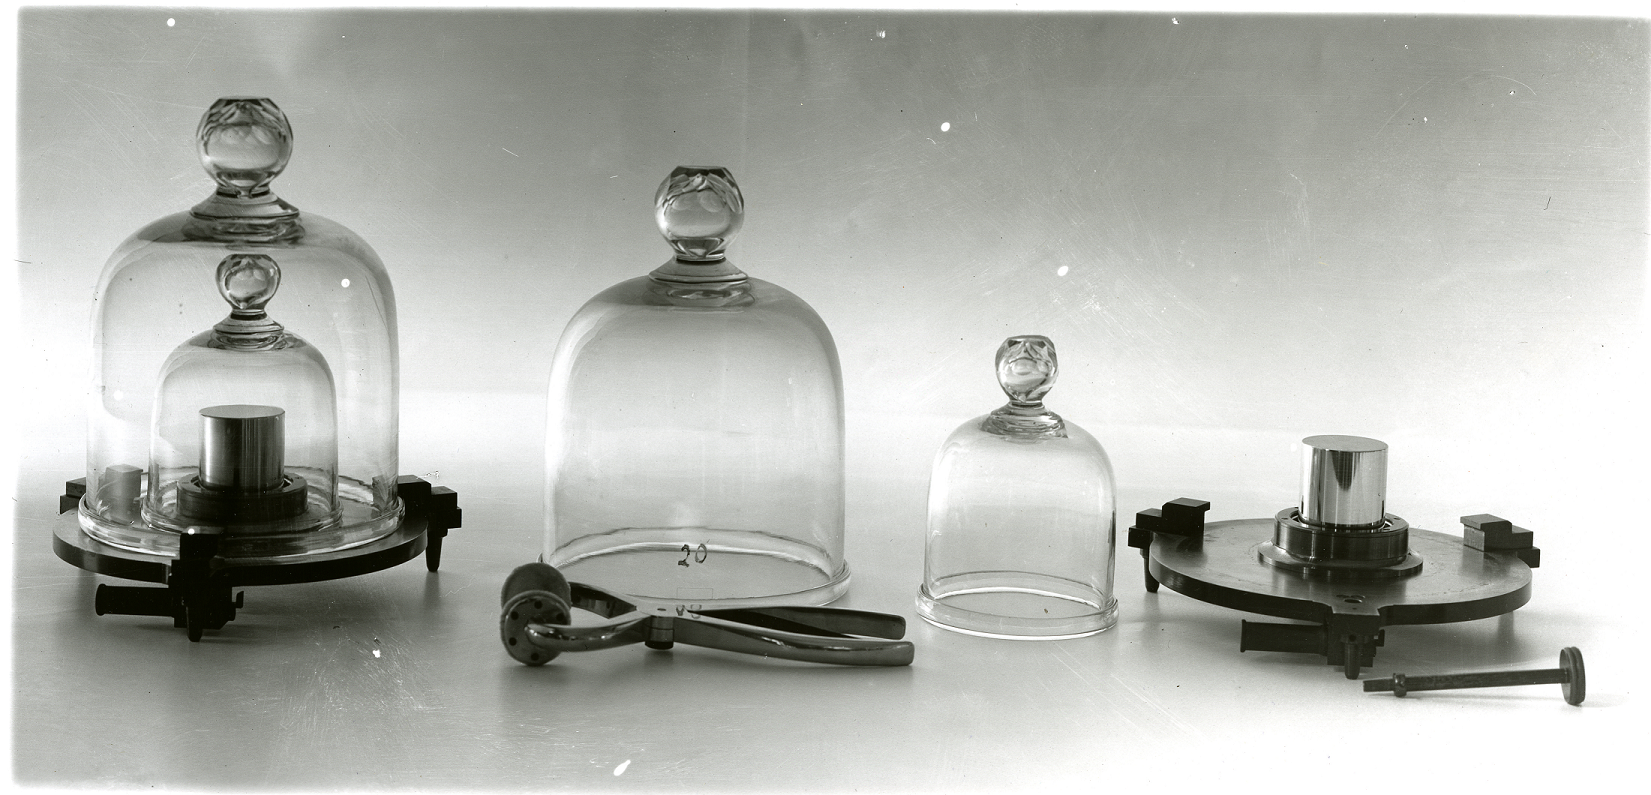
\includegraphics[width=\textwidth]{images/kilogram}

{\tiny \href{https://commons.wikimedia.org/wiki/File:MassStandards_005.jpg}{Image Source: Wikimedia}, Public Domain}
}

\againframe<2-3>{challenges3}


\frame{
\frametitle{Precise}
{\small Synonyms: certain, exact, specific, low variance}\\

\begin{center}
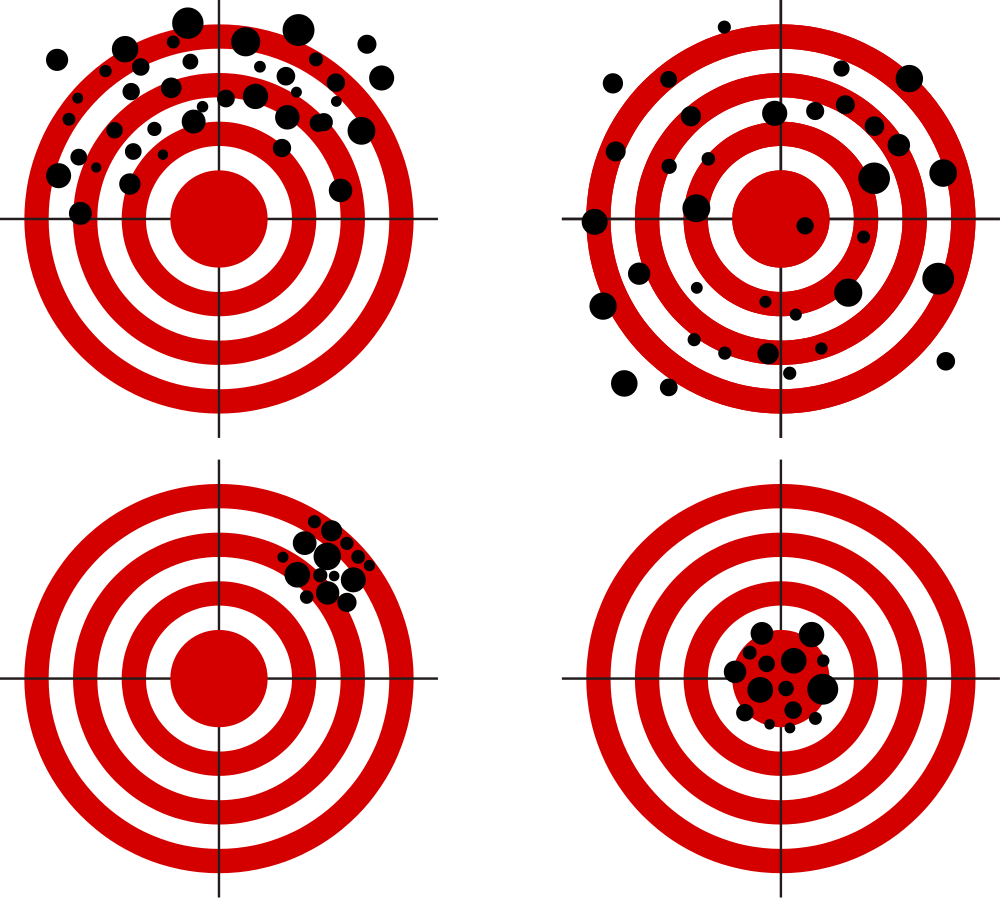
\includegraphics[width=0.6\textwidth]{images/accuracyprecision}
\end{center}

\vspace{-1em}
{\tiny \href{https://commons.wikimedia.org/wiki/File:Reliability_and_validity.svg}{Image Source: Wikimedia}, Nevit Dilmen}
}


\againframe<3-4>{challenges3}


\frame{
\frametitle{Reliable}
{\small Synonyms: dependable, replicable, repeatable, consistent}\\

\vspace{1em}

Typically used in the context of:

\begin{itemize}
\item Multiple measures used in a scale % scale reliability
\item Multiple scores at different times % test-retest reliability 
\item Multiple individuals coding using one method % inter-coder/inter-rater reliability
\end{itemize}

}

% Multiple measures


\frame{\huge\vskip20pt\textbf{Questions?}}


\frame{
\frametitle{Key Points}

\begin{enumerate}\itemsep1em
\item Theory is about concepts
\item Analysis is about measured variables
\item So our task as scientists is to:
	\begin{itemize}
	\item Find observable implications of theory
	\item Draw theoretical implications from measures
	\end{itemize}
\end{enumerate}
}


\appendix
\frame{}

\end{document}
